%-----------------------------------------------------
% Chapter: Prototype Implementation
%-----------------------------------------------------
\chapter{Implementation}
\label{chap:implementation}
Implementation of the project predominately utilised the  Python\footnote{https://www.python.org/} programming language. The motivation for using Python originated from prior familiarity with the language, and it's collection of machine learning and web development libraries which form two key components of the project. Though Python allows for relatively quick development, its known drawback of speed was a cause of concern.

\noindent
\newline
As stated in \autoref{chap:requirements_analysis}, in research, model training time is often neglected in favour of high performing models. As this project involves the creation of a prototype software application, it was important that the impact of model training time on overall development was minimal.

\noindent
\newline
This chapter describes the development process for implementing the CoVeR algorithm, the language and text classification models as well as the SONGIFAI web application. 

\section{Hardware Specification}
All implementation was completed on a personal machine. The hardware specifications for the machine are highlighted below

\begin{table}[h!]
	\centering
	\begin{tabular}{||c | c||} 
		\hline
		Hardware Component & Specification \\ [0.5ex] 
		\hline\hline
		CPU & Intel Core i7-8750H CPU @ 2.20GHz x 12 \\ 
		GPU & NVIDIA GeForce GTX 1050 Ti 4GB \\
		RAM & 16GB \\
		\hline
	\end{tabular}
	\caption[Hardware Specification]{Hardware specification for machine used throughout development}
	\label{table:1}
\end{table}
\section{Calculating Co-occurrence Statistics}
Many unsupervised NLP methods compute co-occurrence statistics before learning takes place. Typically, co-occurrence statistics, such as GloVe's word-word co-occurrence matrix contain sparse data, and computing them can often be a computationally more expensive task than the learning itself. The original GloVe paper describes this process as a \textit{'one-time upfront cost'}, with the assumption that selected corpora are static. Unfortunately, for many NLP pipelines such corpora are more dynamic in nature. For example, social data from online platforms such as Twitter\footnote{https://twitter.com/} are in constant flux and relying on pre-computed co-occurrence statistics to learn Twitter based word embeddings is sub-optimal. Compared to GloVe, computing the co-occurrence statistics for CoVeR has added complexity due to the transition from a co-occurrence matrix to a co-occurrence tensor.

\noindent
\newline
Attempts to efficiently compute co-occurrence counts include the usage of distributed computing techniques such as \textit{MapReduce} (\cite{Lin2008}, \cite{Wittek2013}). MapReduce is a model for distributed computing which at its crux involves two functional processes: \textit{map} and \textit{reduce}. During the map process, data is taken in as key/value pairs and transformed into intermediary key/value pairs. These are then passed to the reduce process which aggregates data which share the same key. An example MapReduce process is walked through in \autoref{fig:fig14} below. 

\begin{figure}[h]
	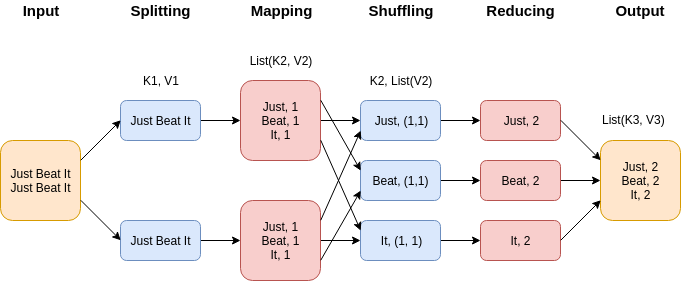
\includegraphics[width=14cm, height=6cm]{./figures/fig14}
	\centering
	\caption[MapReduce Word Count Example]{MapReduce word count example:}
	\label{fig:fig14}
\end{figure}
\noindent
Apache Spark is an open-source framework, written in Scala, for distributed computing and has recently emerged as the de-facto choice for big data processing over Apache Hadoop. Like Hadoop, Spark also supports the MapReduce programming paradigm but boasts features such as enhanced speed, a distributed data structure, as well as API's written in multiple programming languages. Spark uses a master/slave architecture to achieve distributed computing. The \textit{driver} acts as the master node and distributes tasks to many different worker nodes, also known as \textit{executors}, which each run their own JVM processes to execute tasks.

\begin{figure}[h]
	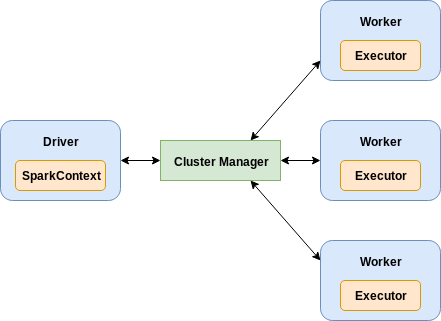
\includegraphics[width=8cm, height=5cm]{./figures/fig19}
	\centering
	\caption{High level view of the Spark Architecture. The spark context is where the main program is defined, which is then split into tasks to be completed via numerous executors.}
	\label{fig:fig19}
\end{figure}

\noindent
\newline
PySpark, a Python API for Spark was initially to pre-process and calculate co-occurrence counts for the dataset. 
Unfortunately, the overhead of collecting completed executor tasks to the driver as well as the cross language communication between Python and Scala made PySpark an unfavourable option for collecting co-occurrence counts. A similar parallelised approach which avoided cross language communication involved the use of Python's multiprocessing module. However this method suffered from Pythons Global Interpreter Lock (GIL) which prevents shared access of Python objects across multiple threads. Taking inspiration from GloVe's original implementation, which is written in C, Cython, an extension of Python, was used to quickly process co-occurrence counts.

\noindent
\newline
Cython is a superset of the Python programming language which aims to provide C like performance whilst maintaining the ability to write Python like code. Native Python programs can experience major speed improvements using Cython because of its ability to compile Python to C code. Ultimately, calculating the co-occurrence statistics for CoVeR was achieved using Cython which provided major speed ups compared to the parallelised approaches outlined before. To highlight these gains, the implementation was compared against its Python equivalent, as well as a commonly used Python implementation of GloVe, developed by Simon Grady\footnote{https://github.com/GradySimon/tensorflow-glove}. This can be seen in \autoref{fig:fig15}.

\begin{figure}[ht]
	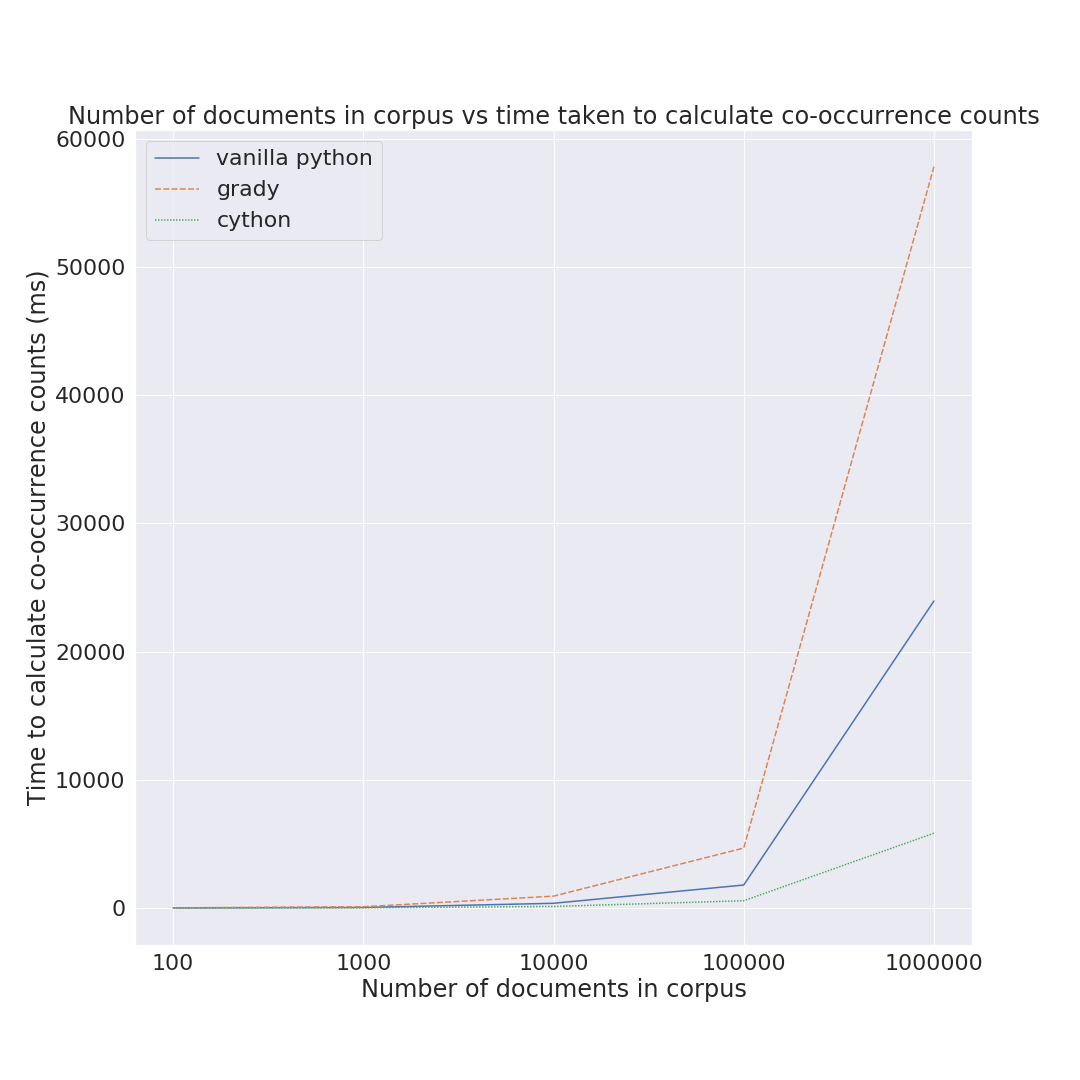
\includegraphics[width=13cm, height=13cm]{./figures/fig15}
	\centering
	\caption[Co-occurrence benchmarks]{A comparison of  }
	\label{fig:fig15}
\end{figure}

\noindent
\newline
\section{CoVeR Implementation}
At time of writing, no public implementation of CoVeR is available. As a result and to meet the needs of this project, CoVeR was implemented using the PyTorch library. PyTorch is a Python library based on Torch, which supports Numpy like operations which can be accelerated through the GPU. The training parameters are highlighted in \autoref{Tab:coverparams} .
\begin{table}[h!]
	\centering
	\begin{tabular}{||c | c||} 
		\hline
		Hyperparameter & Value \\ [0.5ex] 
		\hline\hline
		Embedding Size & 50 \\ 
		Window Size & 8 \\
		Batch Size & 512 \\
		Epochs & 10 \\
		Optimiser & Adam \\
		Subsample Threshold & 0.05 \\
		\hline
	\end{tabular}
	\label{Tab:coverparams}
	\caption[CoVeR Hyperparameters]{CoVeR Hyperparameters}
\end{table}
\section{Model Implementations}
Implementation of the language models and text classifier was done using Keras. Keras is a high level machine learning library written in Python, which runs on top of either Tensorflow or Theano. The motivation behind using Keras comes from its ease of use to quickly develop deep learning networks. In this project Keras is deployed using Tensorflow as a backend, specifically for its GPU capabilities. As stated in \autoref{chap:data_methodology}, the architectural structure of the language models and the text classifier was the same. From an implementation standpoint differences occurred in the number of hidden units for the LSTM used, as well as the size of the inputs into the network. 



\section{SONGIFAI}
\subsection{Architecture}
SONGIFAI, the prototype system takes the form of a web application. Typically the development of such systems follows the model-view-controller (MVC) paradigm, where the model represents application state, the view presents the state to the user and the controller interfaces between the two. For this prototype, the MVC design pattern was followed. The overall SONGIFAI system architecture can be seen in \autoref{fig:songifaiarc} and screenshots of the application can be found in \autoref{app:screen}.
\begin{figure}[ht]
	\centering
	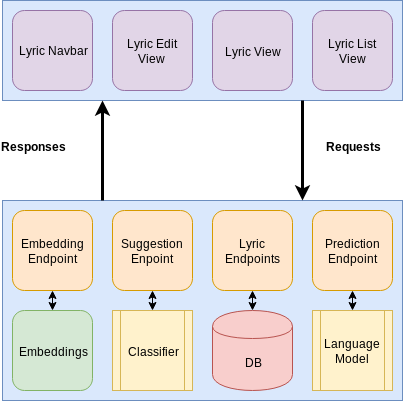
\includegraphics[width=8cm, height=8cm]{./figures/fig22}
	\caption[SONGIFAI Architecture]{SONGIFAI Architecture}
	\label{fig:songifaiarc}
\end{figure}

\subsubsection{Client Side}
For the client side development of SONGIFGAI, requirement NFR1 states that the system must take the form of a web application. However, being a prototype solution, it was important that development was swift and well structured so that the research goals of the project were not hindered. To help achieve this, ReactJS was chosen as the front-end development framework.

\noindent
\newline
ReactJS, (simply known as React) is a JavaScript framework for building user interfaces originally developed and maintained by Facebook. A key concept in React is the idea of components which all React user interfaces are composed off. Simply put a React component takes properties as input and outputs a UI using those properties. Comparable to the object oriented programming paradigm, React promotes the reuse of code through high modularized components.

\subsubsection{Server Side}
Requirement FR1 refers to a user of the system being able to save, load and edit their lyrics. Moreover for easy compatibility with Keras generated models, another Python based library was used for server side development. Django is a python based web framework which follows the model-view-template (MVT) architectural pattern(REF), although for this project it was adapted to the MVC pattern due to the user interface being handled by React. Out the box, Django comes with a configured database, an administration panel, and simple mechanism to create restful endpoints. These were very favourable for the swift development of the prototype system.

\noindent
\newline
Both the client and server were developed in Docker containers, which allow for easy deployment to hosted services. As this was a prototype application, actual deployment was not considered, though the mechanisms are in place for easy future deployment. 